%%%%%%%%%%%%%%%%%%%%%%%%%%%%%%%%%%%%%%%%%
% Beamer Presentation
% LaTeX Template
% Version 1.0 (10/11/12)
%
% This template has been downloaded from:
% http://www.LaTeXTemplates.com
%
% License:
% CC BY-NC-SA 3.0 (http://creativecommons.org/licenses/by-nc-sa/3.0/)
%
%%%%%%%%%%%%%%%%%%%%%%%%%%%%%%%%%%%%%%%%%

%----------------------------------------------------------------------------------------
%	PACKAGES AND THEMES
%----------------------------------------------------------------------------------------

\documentclass{beamer}

\mode<presentation> {

% The Beamer class comes with a number of default slide themes
% which change the colors and layouts of slides. Below this is a list
% of all the themes, uncomment each in turn to see what they look like.

%\usetheme{default}
%\usetheme{AnnArbor}
%\usetheme{Antibes}
%\usetheme{Bergen}
%\usetheme{Berkeley}
%\usetheme{Berlin}
%\usetheme{Boadilla}
%\usetheme{CambridgeUS}
%\usetheme{Copenhagen}
%\usetheme{Darmstadt}
%\usetheme{Dresden}
%\usetheme{Frankfurt}
%\usetheme{Goettingen}
%\usetheme{Hannover}
%\usetheme{Ilmenau}
%\usetheme{JuanLesPins}
%\usetheme{Luebeck}
\usetheme{Madrid}
%\usetheme{Malmoe}
%\usetheme{Marburg}
%\usetheme{Montpellier}
%\usetheme{PaloAlto}
%\usetheme{Pittsburgh}
%\usetheme{Rochester}
%\usetheme{Singapore}
%\usetheme{Szeged}
%\usetheme{Warsaw}

% As well as themes, the Beamer class has a number of color themes
% for any slide theme. Uncomment each of these in turn to see how it
% changes the colors of your current slide theme.

%\usecolortheme{albatross}
%\usecolortheme{beaver}
%\usecolortheme{beetle}
%\usecolortheme{crane}
%\usecolortheme{dolphin}
%\usecolortheme{dove}
%\usecolortheme{fly}
%\usecolortheme{lily}
%\usecolortheme{orchid}
%\usecolortheme{rose}
%\usecolortheme{seagull}
%\usecolortheme{seahorse}
%\usecolortheme{whale}
%\usecolortheme{wolverine}

%\setbeamertemplate{footline} % To remove the footer line in all slides uncomment this line
%\setbeamertemplate{footline}[page number] % To replace the footer line in all slides with a simple slide count uncomment this line

%\setbeamertemplate{navigation symbols}{} % To remove the navigation symbols from the bottom of all slides uncomment this line
}

\usepackage{graphicx} % Allows including images
\usepackage{booktabs} % Allows the use of \toprule, \midrule and \bottomrule in tables
\usepackage{verbatim}
%----------------------------------------------------------------------------------------
%	TITLE PAGE
%----------------------------------------------------------------------------------------

\title[Homogeneity test via VLMC training]{Time series homogeneity test via VLMC training} % The short title appears at the bottom of every slide, the full title is only on the title page

\author{Xin Li} % Your name
\institute[Northeastern University] % Your institution as it will appear on the bottom of every slide, may be shorthand to save space
{
Northeastern University \\ % Your institution for the title page
\medskip
\textit{} % Your email address
}
\date{} % Date, can be changed to a custom date

\begin{document}

\begin{frame}
\titlepage % Print the title page as the first slide
\end{frame}

\begin{frame}
\frametitle{Introduction} % Table of contents slide, comment this block out to remove it

\begin{itemize}
\item Modeling random processes
as full n - Markov Chains (MC)  can be inadequate, if $n$ is small, and over-parameterized
for large $n$.
\item If say, the cardinality of the base state space
is four, n=10, then the number of parameters is around 3.1 million.
\item The
popular since sixties Box-Jenkins ARIMA approach in quality control
is inadequate in
linguistics, genomics and proteomics, security, etc, where
comparatively long {\bf non-isotropic contexts are important for prediction} leading to
huge memory size of the full n-Markov Chain (MC).

\end{itemize}

\tableofcontents % Throughout your presentation, if you choose to use \section{} and \subsection{} commands, these will automatically be printed on this slide as an overview of your presentation
\end{frame}
%-------------------------------------------------
%-------------------------------------------------
\begin{frame}
\frametitle{Introduction} % Table of contents slide, comment this block out to remove it

\begin{itemize}
\item Popularity of  sparse Variable memory Length MC (VLMC), is
increasing rapidly after {\bf J. Rissanen}  constructed  in 1983   {\bf stochastic suffix tree} by algorithm {\bf `Context'}  for compression and proved its consistency under stationarity with exponential mixing.. 

 \item  The  VLMC main idea: the probability
 of each symbol only depends on a {\bf finite part of the total past n-string}. The {\bf length
of this relevant `context' is a function of the past itself}. This can drastically {\bf cut the number of parameters} of the full n-MC.

\item
J. Ziv (2011)  shows: If the training string  cannot be treated as a realization of a stationary ergodic process (as in Genomics and Proteomics), then  the algorithms worked out for constructing   suffix tree can be used for more robust similarity tests without stationarity and even without randomness assumptions.

\end{itemize}

\tableofcontents % Throughout your presentation, if you choose to use \section{} and \subsection{} commands, these will automatically be printed on this slide as an overview of your presentation
\end{frame}
%-------------------------------------------------
%-------------------------------------------------
\begin{frame}
\frametitle{}
Sparse VLMC over alphabet  $A$  (`letters') is a very special case of $n$-MC. 
\noindent $n$ is the maximal length of {\bf contexts}. A context
 \begin{equation}
 C(x_0) = x_{-1},\dots,x{{-k}}, k\le n: = x_{-1}^{-k}, x_i\in A
 \end{equation}
  (to a current state $x_0$) is a subsequence of the past states $x_{-1}^{-n}$ of the {\bf minimal length} such that the conditional probability satisfies:
  \begin{equation}
  P(x_0)|x_{-1}^{-m})\equiv P(x_0)|x_{-1}^{-k}) ,  \forall m>k.
  \end{equation}

For large $n$, VLMC is sparse, if the total number of contexts ${\cal C}(n)$ is polynomial in $n$, informally, if
  ${\cal C}(n)<< 2^n$.
  VLMC can be viewed as probability suffix tree, 
  {\bf an illustrative example of stochastic context tree is on the next slide}.

\end{frame}
%-------------------------------------------------
%-------------------------------------------------
\begin{frame}
\frametitle{Figure}
\begin{figure}[h!]
  \centering
      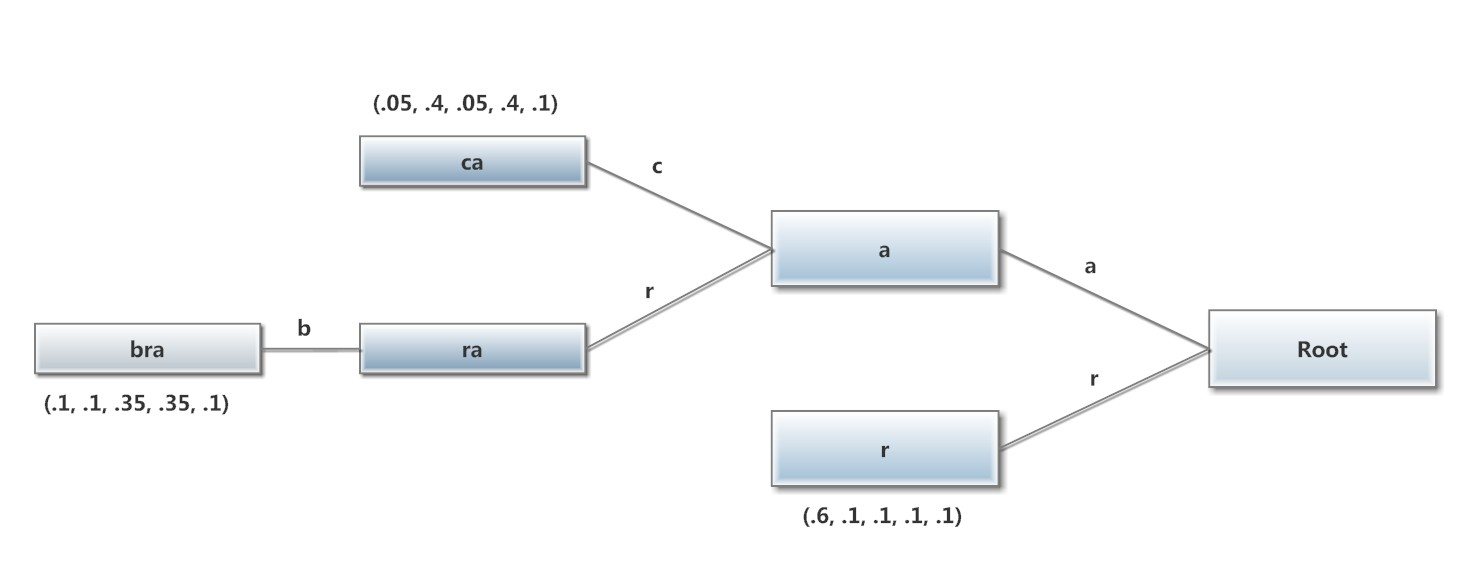
\includegraphics[scale=0.30]{ContextTree.jpg}
  \caption{Illustrative example of stochastic context tree with distributions of the root given contexts written under the leaves of the tree}
\label{fig:ContextTreeExample}
\end{figure}
\end{frame}
%-------------------------------------------------
%-------------------------------------------------
\begin{frame}
\frametitle{}
 \begin{itemize}


\item Testing proximity between non-stationary proteins used either likelihood comparisons (G. Bejeranol, 2003 ), or equally unjustified messy  {\bf test BB} on stochastic suffix trees (Balding, Bush et al, 2008) generated by `Context' or alternative algorithm PST of `Probability Stochastic Tree'.

\item If a universal compressor such as zip (LZ - 78) compresses efficiently the LONG presumably stationary training string (such as literary text),  then the homogeneity {\bf CCC - test} with its theory developed by us two years ago is a computationally simple efficient substitute for test BB and likelihood-based tests.\


 \item Approximated  {\bf Likelihood Ratio test}  for query vs. simulated training strings {\bf given the `frozen' stochastic suffix tree of the training string} is proposed here.\
\end{itemize}
\end{frame}

%-------------------------------------------------
%-------------------------------------------------
\begin{frame}
\frametitle{}
\begin{itemize}
\item Our test VLMClr is the Studentized sum of empirical log-likelihood ratios between the  query slices and simulated  training string continuation of the same length. We prove {\bf exponential tails optimality} and {\bf asymptotic normality of our test} similarly to our study of the CCC-test.

\item We find the frequencies of all contexts in slices of training and query texts.

\item  One of major additional advantages of VLMClr over CCC is its more straightforward use for the follow up estimation of contexts contributing the most to the discrimination between strings distributions (styles of authors or different regions of data strings) which were previously shown to be distinct. This is crucial for convincing linguists or biologists, who are generally skeptical about statistical string processing.\
\end{itemize}
\end{frame}

%-------------------------------------------------
%-------------------------------------------------
\section{Madison vs Hamilton discrimination of styles}
\begin{frame}
\frametitle{}
\begin{itemize}
\item The {\bf Federalist Papers} written by Alexander Hamilton, John Jay and
James Madison appeared in newspapers in October 1787-August 1788 for
persuading the citizens of the State of New York to ratify the U.S. 
Constitution. Seventy seven essays first appeared in several
different newspapers all based in New York and then eight additional
articles written by Hamilton on the same subject were published in a
booklet form. 
\item  The
authorship of 12 papers (Df, No. 49-58, 62,63) has
been in dispute; these papers are usually referred to as the
disputed papers. It has been generally agreed that the Df-papers
were written by either Madison or Hamilton, without consensus on
particulars.
\item  All previous stylometry attributors have given all Dfs to Madison.
\end{itemize}
\end{frame}

%-------------------------------------------------
%-------------------------------------------------
\begin{frame}
\frametitle{}
 Our goal
was answering the 3 questions:

1. Is VLMC- methodology
 attributing all Mf to Madison and 

2.  rejects significantly identity of the Hf style
 to that of Mf ?

 3. What contexts are most statistically different in Mf and Hf?

 Answers are: yes on first questions: Mf  were
attributed to Madison,  Hf and Mf identity of styles was rejected.


\end{frame}
%-------------------------------------------------
%-------------------------------------------------
\begin{frame}
\frametitle{}
First, we combine all 14 Madison's article into one file and use it as the
training data. The cutoff number $n$ is set to be 15 (thus at most
15 {\it letters} decide about the next letter)\


\begin{table}[h!]
\caption{Variable Length Markov Chain Training Result:} 
\centering
\begin{tabular}{ l | c  }
    \hline

    alphabet  & '*abcdefghijklmno\\
&pqrstuvwxyz' \\ \hline
    number of alphabet &  27 \\ \hline
    number of letters &  228744 \\ \hline
    maximal order of Markov chain & 13 \\ \hline
    context tree size & 3365 \\ \hline
    number of leaves & 2353\\ \hline
    AIC & 644816 \\ \hline
  \end{tabular}
\end{table}


\end{frame}
%-------------------------------------------------
%-------------------------------------------------
\begin{frame}
\frametitle{Intra VLMC test}
 We use each slice of Madison's data as query
string and use the remaining 8 slices as training string. We want to
compute the log-likelihood of each query string.\\

\begin{table}[h!]
\caption{Inter-loglikelihood output} % title of Table
\centering
\begin{tabular}{c c c c} % centered columns (4 columns)
\hline % inserts single horizontal line
-27863.56 &-28047.04 &-27236.75 &-26559.74 \\
-24995.70 &-27173.49& -26209.20 &-25182.81 \\
-25622.52\\
\hline %inserts single line
\end{tabular}
\end{table}


\end{frame}
%-------------------------------------------------
%-------------------------------------------------
\begin{frame}
\frametitle{}
Hamilton's article has 152496 letters. We cut the letters into 6 slices so
that each
slice contains 25416 letters ( 25416x6=152496 )\\
\par Last, do the inter-VLMC test. Use the total training result of Madison to
predict the log-likelihood of each slice of Hamilton.\\
\begin{table}[h!]
\caption{Intra-loglikelihood output} % title of Table
\centering
\begin{tabular}{c c c c} % centered columns (4 columns)
\hline % inserts single horizontal line
 -28552.20 &-28462.64 &-28511.57 &-28234.03 \\
-27227.31 &-26510.97\\

\hline %inserts single line
\end{tabular}
\end{table}


\end{frame}
%-------------------------------------------------
%-------------------------------------------------
\begin{frame}
\frametitle{}
 The mean value of these 9 log-likelihood is -27916.45
 The variance of these 9 log-likelihood is 721562.6\\

 Use the formula to do test:
$$t=\frac{\l_{1}-\l_{2}}{\sqrt{var_{1}/n_1+ var_{2}/n_2}}$$

Plug in the numbers and we get the t-value  2.690809\\


\end{frame}
%-------------------------------------------------
%-------------------------------------------------
\begin{frame}
\frametitle{}
\par Finally, to check consistency of our discrimination  we also did a comparison between
Madison itself. (we suppose to have a t-value around 0)\\
\par The inter VLMC of Madison vs Madison log-likelihood result:\\
\begin{table}[h!]
\caption{Inter-loglikelihood output} % title of Table
\centering
\begin{tabular}{c c c c} % centered columns (4 columns)
\hline % inserts single horizontal line
 -27725.26 & -27341.10 & -26948.34 &-26352.83 \\
-23933.95& -26703.40& -25770.18& -24609.77\\
-25525.76\\

\hline %inserts single line
\end{tabular}
\end{table}


\end{frame}
%-------------------------------------------------
%-------------------------------------------------
\begin{frame}
\frametitle{Federalist papers discrimination : Madison vs Hamilton}


Combine all 14 Madison's article into one file and use it as the
training data. The cutoff number $n$ is set to be 15 (sequence of at most 15 {\it English letters or space}
decide the next letter).

\par Run the `Context' software in R (M\"{a}chler and P. B\"{u}hlmann, 2004) for training VLMC of Madison.
Divide Hamilton papers into several
slices of equal size, find the log-likelihood of each query (Hamilton) slice. T-test rejects style homogeneity of the two authors for
selected three slice sizes with t-values from 3 to 4.  No. of Contexts is around 2400 as compared to $(27)^{15}$.


{\bf Follow up}: For each context found in training VLMC of each author, calculate its mean number of occurrences.
Cut Madison/Hamilton data into respectively 9/6, 14/9 and 20/14 slices to compare results stability. Finally, we calculate
the t-value for occurrence differences for each VLMC context, order them and find the most significant.\




\end{frame}
%-------------------------------------------------
%-------------------------------------------------
\begin{frame}
\frametitle{Madison vs Hamilton}
\begin{itemize}
\item The VLMC significantly different contexts appear in all 9/6, 14/9 and 20/14 slices with p-value $<0.01$:

\item Patterns that Madison uses more frequently than Hamilton:

*bo , *el , *on*t , *on*th , *th , ay*b , ay*be , bot , both , by , by* , by*o , by*t , d* , d*on , de* , der* , e* , ed*b , ese* , eside , ewe , f* , fore* , g*the* , han* , he*n , ix , ixe , kscgr* , lst , lt* , nd*be , orm



\item Patterns that Hamilton uses more frequently than Madison:

*at , *at* , *nat , *ther , *this* , *to , *to* , *up , *wo , ces , ct , dic , duc , e*ar , e*to* , erac , es*of* , eso , ies , ilit , ity* , lit , nati , nation , ne , om , ont , ontr


\item In our  discrimination we used the software
developed by M\"{a}chler and described in his popular tutorial with B\"{u}hlmann.
\end{itemize}


\end{frame}
%-------------------------------------------------
%-------------------------------------------------
\section {Nasdaq data} 
\begin{frame}
\frametitle{Nasdaq data}
We use historical {\bf Nasdaq data} on multivariate daily returns for almost 498
days from April 4th 2011 to March 27th 2013 collected from $finance.yahoo.com$ and converted into
log-returns. We reduce the dimensionality of single-day returns via MatLab version of
the principal component analysis (PCA) and compress the data set
to the sequence of first (either two or three) Principal Components (PC)
describing a major part of the data variability, see figure ~\ref{fig:SigularValuesOfDailyReturns}. We fit
their VLMC stochastic model and apply it for discrimination between statistical properties of different parts of
the data.




\end{frame}
%-------------------------------------------------
%-------------------------------------------------
\begin{frame}
\frametitle{Fiture}
\begin{figure}[h!]
  \centering
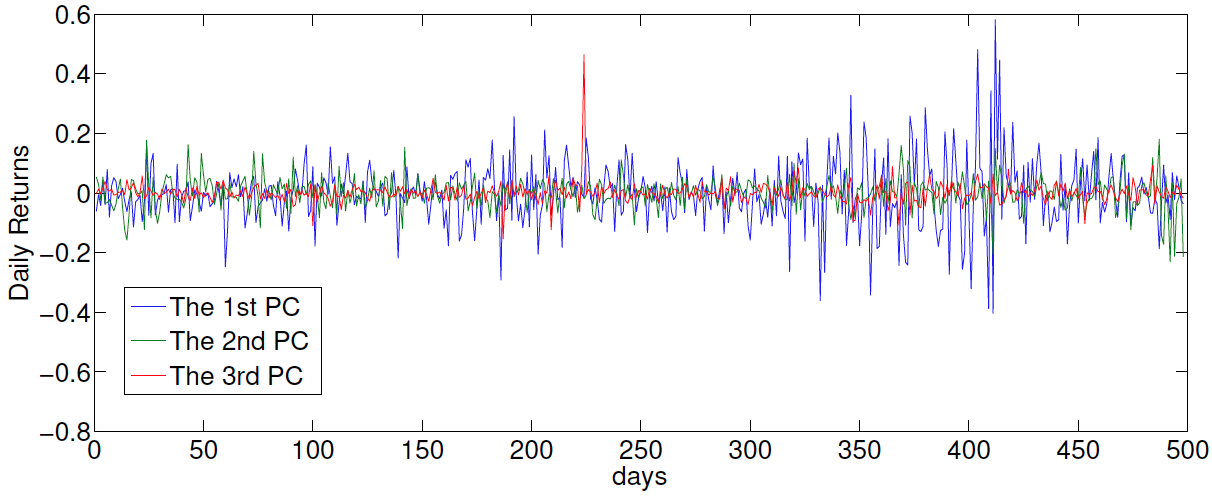
\includegraphics[scale=0.29]{FirstThreeDailyReturns.png}
\label{fig:3PcDailyReturns}
  \caption{Three PC of daily returns}
\end{figure}


\end{frame}
%-------------------------------------------------
%-------------------------------------------------
\begin{frame}
\frametitle{}
\begin{figure}[h!]
  \centering
      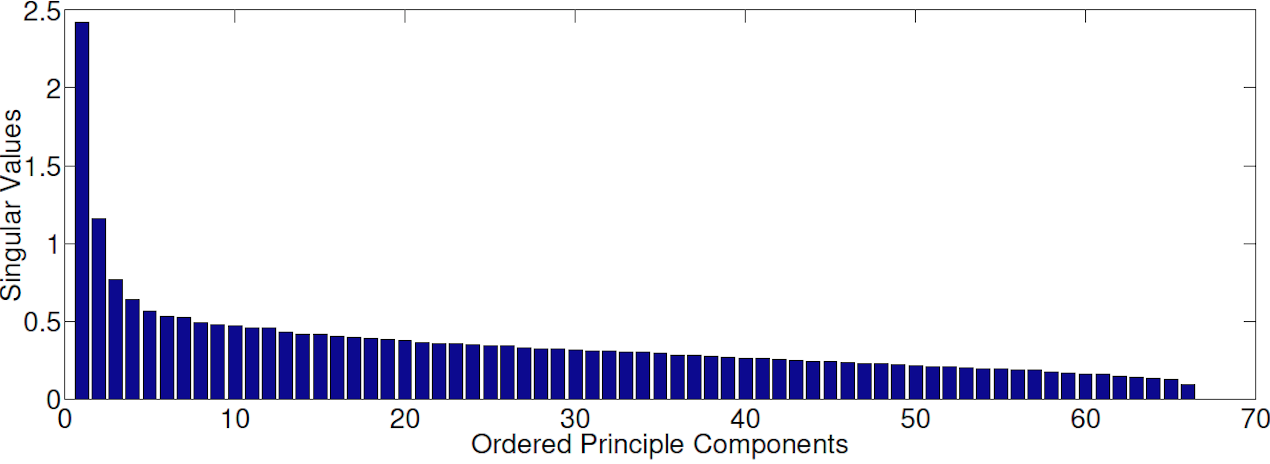
\includegraphics[scale=0.27]{SingularValuesReturns.png}
  \caption{Singular values of daily returns}
\label{fig:SigularValuesOfDailyReturns}
\end{figure}


\end{frame}
%-------------------------------------------------
%-------------------------------------------------
\begin{frame}
\frametitle{Results for 3 PCs}
First, the range of each PC is divided into three equal intervals (bins) . Triples of PC-values are
compressed to triples of  integers from set \{1,2,3\} according to their belonging to corresponding
bins and their triples are labeled with 26
English letters from A to Z or the * symbol. 


\end{frame}
%-------------------------------------------------
%-------------------------------------------------
\begin{frame}
\frametitle{}
Only 8 of all 27 symbols were observed in the whole sequence.

The homogeneity t-test between 1-150 and 301-420 (quiet and volatile
regions)
trained on 301-420, cutting into 12 slices. The t-score is 0.1419433.\\

\begin{table}[H]
\caption{ Variable Length Markov Chain Training Result:} 
\centering
\begin{tabular}{l | c  }
    \hline
    alphabet  & 'bdejkntw' \\ \hline
    number of alphabet &  8 \\ \hline
    number of letters &  120 \\ \hline
    maximal order of Markov chain & 2 \\ \hline
    context tree size & 7 \\ \hline
    number of leaves & 5\\ \hline
    AIC & 315.7 \\ \hline
  \end{tabular}
\end{table}

\end{frame}
%-------------------------------------------------
%-------------------------------------------------
\begin{frame}
\frametitle{}
\begin{table}[h!]
\caption{Inter-loglikelihood output} % title of Table
\centering
\begin{tabular}{c c c c} % centered columns (4 columns)
\hline % inserts single horizontal line
-5.109994  &-8.113694 &-11.494689 & -5.622557 \\
 -5.109994  &-5.199606  &-5.020382  &-8.624520  \\
-6.135120  &-5.109994  &-8.022345  &-4.507818  \\
 -5.109994  &-5.622557 & -4.374287 \\
\hline %inserts single line
\end{tabular}
\end{table}


\end{frame}
%-------------------------------------------------
%-------------------------------------------------
\begin{frame}
\frametitle{}
\begin{table}[h!]
\caption{Intra-loglikelihood output} % title of Table
\centering
\begin{tabular}{c c c c} % centered columns (4 columns)
\hline % inserts single horizontal line
   -6.224733 &  -6.135120 & -5.622557 & -5.622557\\
 -10.284486 &-10.012552 &-10.144724 &-10.347058\\  
-7.736400 & -6.498026 &  -9.982415 & -9.603383\\
\hline %inserts single line
\end{tabular}
\end{table}




\end{frame}
%-------------------------------------------------
%-------------------------------------------------

\begin{comment}
\begin{frame}
\frametitle{Prediction accuracy}
\par We estimate the Squared Bias to show the accuracy of our prediction by predicting 10 consecutive 
letters from the 131st to 140th and for each letter, the prediction is based on training previous 130 letters. 
The variance of the log-likelihood of the simulated letters is 0.3947234. The Squared Bias is 0.04815128 which is 8.1 times less. This shows adequacy of our prediction.

Also, we predict each of 20 letters of the quiet zone by training
VLMC on 120 preceding letters. The coincidence rate of predicted and
actual letter was about 75 per cent.




\end{frame}
\end{comment}
%-------------------------------------------------
%-------------------------------------------------
\begin{frame}
\frametitle{}

In the 2-PC case, the quiet region has the pattern L (indicating
that the first PC-value is located in the second bin and the
second PC-value is located in the third bin) and H (indicating
that the first PC-value is located in the third bin and the
second PC-value is located in the second bin) while the
volatile region have the pattern B (indicating that the first
PC-value is located in the first bin and the second PC-value is
located in the second bin) and Q (indicating that the first
PC-value is located in the fourth bin while the second PC-value
is located in the second bin).


\end{frame}
%-------------------------------------------------
%-------------------------------------------------
\begin{frame}
\frametitle{}
In the 3-PC case, the quiet region has the pattern N (indicating that all three PC-values are  located
in the second bin) while the volatile region has the pattern E (indicating that the first PC-value is located
in the first bin while the second and third PC-values are located in the second bin).




\end{frame}
%-------------------------------------------------
%-------------------------------------------------
\subsection{Comparison with GARCH}
\begin{frame}
\par In this subsection, we will make a comparison between our VLMC method and the GARCH model (\cite{GARCH:matlabtoolbox}, \cite{Garch: book}) applied to two different sets of financial data.
\par The first data set we use is the daily log-return data of APPLE Inc. starting from Jan. 2nd, 2009 (Figure ~\ref{fig:AppleDailyReturns}). By observation, we pick the volatile region (the first 450 days returns )and the quiet region (the 500th to 600th days returns) to make a comparison. We first fit the data with the GARCH(1,1) modeled using the MATLAB(R2011a) GARCH toolbox.

\end{frame}

\begin{frame}
\begin{figure}[h!]
\centering
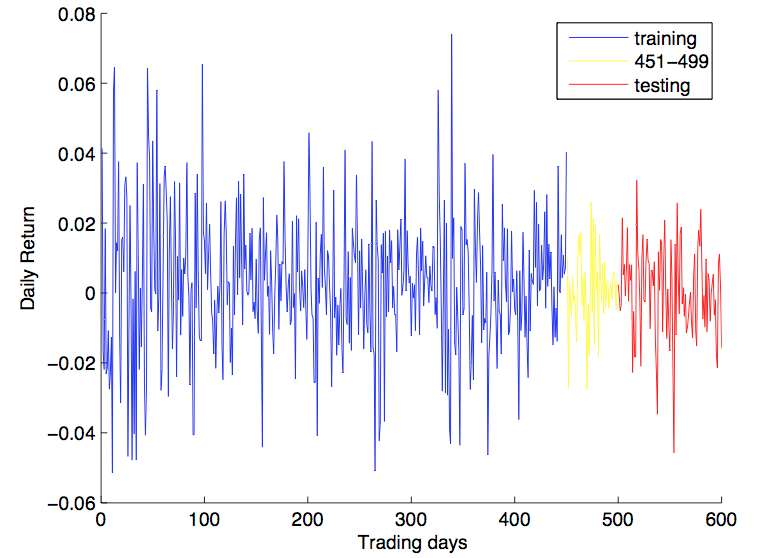
\includegraphics[scale=0.45]{newpic2.png}
\caption[]{Apple Daily Returns}
\label{fig:AppleDailyReturns}
\end{figure}


\end{frame}

\begin{frame}
\begin{eqnarray}
% \nonumber to remove numbering (before each equation)
&y_{t}&= C+\epsilon_{t}\\
&\epsilon_{t}& = \sigma_tz_t \\
&\sigma_t^2& = \kappa+G_1\sigma_{t-1}^2+A_1\epsilon_{t-1}^2
\end{eqnarray}
\par Let $\hat{\alpha}_1$ and $\hat{\beta}_1$ be the estimator for GARCH(1) and ARCH(1) in the first model.
Similar notation can be defined for $\hat{\alpha}_2$ and $\hat{\beta}_2$. From the results, we have $z_1=\frac{\hat{\alpha}_1-\hat{\alpha}_2}{\sqrt{\sigma^2_{\alpha_1}+\sigma^2_{\alpha_2}}}\doteq2.1554$,
and $z_2=\frac{\hat{\beta}_1-\hat{\beta}_2}{\sqrt{\sigma^2_{\beta_1}+\sigma^2_{\beta_2}}}\doteq -1.6971$. The p-values obtained are $p_1$=0.0311 and $p_2$ = 0.0897.

\par We apply the same data on VLMC. The homogeneity t-test between 1-450 and 500-600 (quiet and volatile regions) trained on 1-450 shows that the t-value is -16.02058.
Thus, the p-value $p<0.00001$. This p-value by VLMC is much smaller than the Z-score by GARCH.

\end{frame}

\begin{frame}
\par We also use the {\bf first} principal component of Nasdaq daily log-return data for comparison with GARCH.
Again, let $\hat{\alpha}_1$ and $\hat{\beta}_1$ be the estimator for GARCH(1) and ARCH(1) in the first model.
Similar notation can be defined for $\hat{\alpha}_2$ and $\hat{\beta}_2$. From the results,
we have
$z_1=\frac{\hat{\alpha}_1-\hat{\alpha}_2}{\sqrt{\sigma^2_{\alpha_1}+\sigma^2_{\alpha_2}}}\doteq -1.1798$, and $z_2=\frac{\hat{\beta}_1-\hat{\beta}_2}{\sqrt{\sigma^2_{\beta_1}+\sigma^2_{\beta_2}}}\doteq 2.1554$. And thus, the p-values are $p_1$ = 0.2381 and $p_2$ = 0.0311.

\par We divide the range of the first PC of Nasdaq daily log-returns into 27 bins. Each bin is labeled with 26 English letters from A to Z and symbol *.
The sequence of the first PC of daily log-returns is converted into a sequence of symbols. The homogeneity t-test between 1-150 and 301-420
(quiet and volatile regions) trained on 301-420 shows that the t-value is -7.048379. Thus, the p-value is $p<0.000001$ This p-value by VLMC is much smaller than the p-value by GARCH.




\end{frame}






%-------------------------------------------------
%-------------------------------------------------
\section{Helium emissions and seismic events}
\begin{frame}
\frametitle{Helium emissions and seismic events}
An approximately {\bf 10-year--long set of Helium emissions data from three deep Armenian wells Kadaran, Ararat and Surenavan}, 
the {\bf earthquake dates} in their vicinity shown in our figure 4 was sent to us by Dr. E.A. Haroutunian (Inst. for 
Informatics and Automat. Problems, Armenian Acad. Sci.) 
for our robust analysis. In 
 \cite{IEEEhowto:Haroutunian} they showed separately for each well that the Wilcoxon statistical test distinguishes between quiet 
region of the plot and that preceding strong earthquakes. Wilcoxon test was derived under independence assumption of samples which does not 
hold in this application. Thus our problem was to check if VLMClr can distinguish between the above regions. Instead of separate study of 
data from the three wells we used PCA--compressed data.
The earthquake days from the observations start were 529, 925, 1437, 1797, 1997, 2470, 2629 and 2854.
The singular value plot (figure 5) suggests using either one or 2 PCs.




\end{frame}
%-------------------------------------------------
%-------------------------------------------------
\begin{frame}
\frametitle{}
\begin{figure}[h!]
  \centering
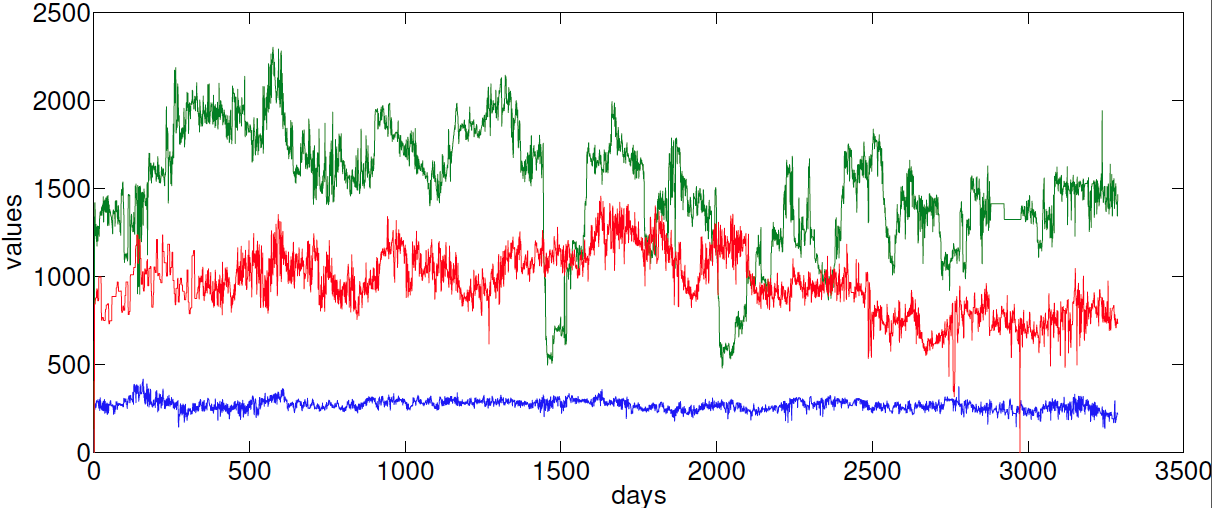
\includegraphics[scale=0.29]{DeepWell.png}
  \caption{Helium emissions data from three deep Armenian wells}
\label{fig:DeepWell}
\end{figure}


\end{frame}
%-------------------------------------------------
%-------------------------------------------------
\begin{frame}
\frametitle{}
\begin{figure}[h!]
  \centering
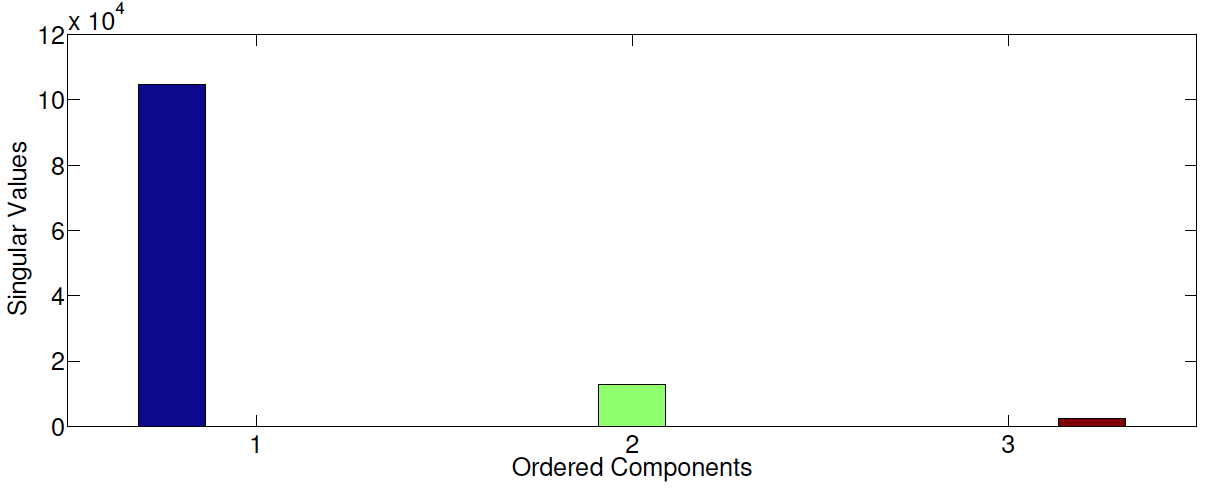
\includegraphics[scale=0.27]{SingularValuesEarth.png}
  \caption{Singular Values}
\label{fig:singularValuesEarth}
\end{figure}


\end{frame}
%-------------------------------------------------
%-------------------------------------------------
\begin{frame}
\frametitle{}
\begin{figure}[h!]
  \centering
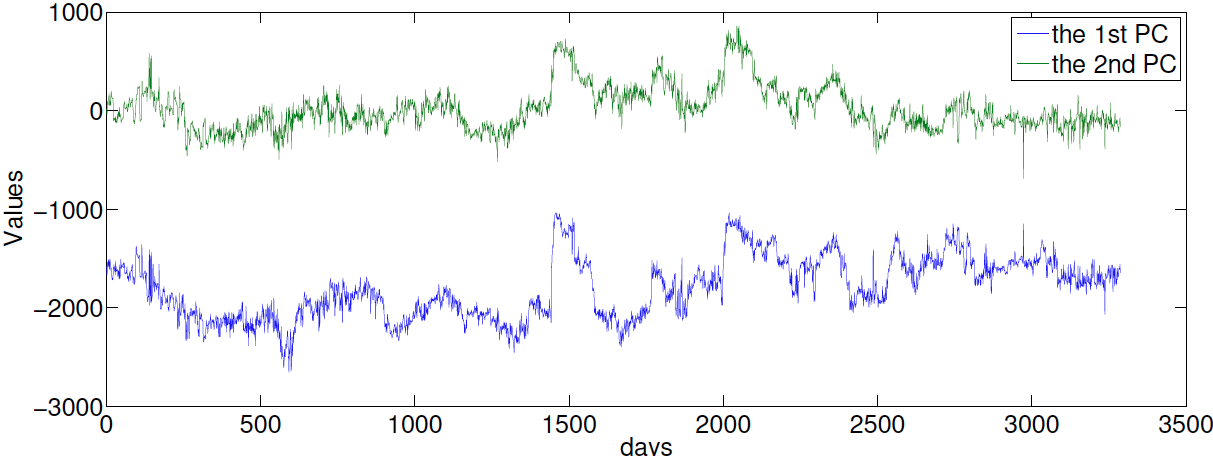
\includegraphics[scale=0.28]{FirstTwoPC.png}
  \caption{Top two principle components}
\label{fig:FirstTwoPC}
\end{figure}


\end{frame}
%-------------------------------------------------
%-------------------------------------------------
\begin{frame}
\frametitle{}
In one--PC case we replaced the continuous PC values with 27 letters from A to Y describing inter $k/(27), 0\le k\le 27$ --locations of 
observations.
The `Context' gave us the following parameters of the stochastic context tree:
\\
\begin{table}[H]
\caption {Variable Length Markov Chain Training Result: }
\centering
\begin{tabular}{ l | c }
    \hline

    alphabet  & 'abfghlmnqrstw' \\ \hline
    number of alphabet &  17 \\ \hline
    number of letters &  400 \\ \hline
    maximal order of Markov chain & 3 \\ \hline
    context tree size & 28 \\ \hline
    number of leaves & 21\\ \hline
    AIC & 1964 \\ \hline
  \end{tabular}
\end{table}




\end{frame}
%-------------------------------------------------
%-------------------------------------------------
\begin{frame}
\frametitle{}
The quiet region 1-400 has the letters "hijklmnopqr", while the volatile region before  and after earthquake 429-568 has the letters "opqrstuvwxy", 
it is impossible to train either region to predict the other one. It is also not necessary to do that because one can easily distinguish different regions 
by observing that the quiet region has the first PC value up above a level "n" (corresponding to a value -1815.101), and the volatile region has the first PC value down below a level "s" (corresponding to a number -2174.363).




\end{frame}
%-------------------------------------------------
%-------------------------------------------------
\begin{frame}
\frametitle{}
In 2--PCs case, the range of each PC is  divided into 5 equal bins. PC-values are
compressed to 5 integers according to their belonging to
bins and their pairs are labeled with 25
English letters from A to Y.
Training the quiet region between 1-400 will provide the following training result:
\begin{table}[h!]
\caption {Variable Length Markov Chain Training Result: }
\centering
\begin{tabular}{ l | c }
    \hline

    alphabet  & 'abfghlmnqrstw' \\ \hline
    number of alphabet &  13 \\ \hline
    number of letters &  400 \\ \hline
    maximal order of Markov chain & 3 \\ \hline
    context tree size & 22 \\ \hline
    number of leaves & 15\\ \hline
    AIC & 1026 \\ \hline
  \end{tabular}
\end{table}







\end{frame}
%-------------------------------------------------
%-------------------------------------------------
\begin{frame}
\frametitle{}
\par The homogeneity t-value between 1-400 (quiet region) and 429-528 (before earthquake) is 4.4 which means that these
two region are quite different. By calculating t-value for each context, we get the context that  distinguishes the most between
these two regions. "l" (the first PC value in the third bin and the second PC value in the second bin)
is the typical pattern of volatile regions before earthquake and "b" (the first PC value is in the first quartile
and the second PC value is in the second quartile) is the typical pattern of quiet region.

\par The homogeneity t-test between 1-400 (quiet region and 529-568 ({\it after} earthquake) is 0.8, which means that we
find not much difference between the quiet region and the region after earthquake. In addition, we find an interesting
letter "c"( it means that the first PC is located in the first bin and the second PC is in the third bin)
which can be an indicator for quiet times to follow because, when  each "c"  appears, there were at least 100 quiet days beyond it in the future.

\end{frame}
%-------------------------------------------------
%-------------------------------------------------


%------------------------------------------------
\section{Reference}
\begin{frame}
\frametitle{References}
\footnotesize{
\begin{thebibliography}{99} % Beamer does not support BibTeX so references must be inserted manually as below

\bibitem{IEEEhowto:Balding}
 D. Balding, P. A. Ferrari,
R. Fraiman,  M. Sued, Limit theorems for sequences of random trees,
, arXiv.org $>$ stat $>$ arXiv:math/0406280, 2007.

\bibitem{IEEEhowto:Bejerano} G. Bejerano, Automata Learning and Stochastic Modeling
for Biosequence Analysis, PhD dissertation, Hebrew University, Jerusalem, 2003.


\bibitem{IEEEhowto:Belloni} A. Belloni and R. I. Oliveira, Approximate group context tree: applications to dynamic programming and dynamic choice models, arXiv.org $>$ stat $>$ arXiv:1107.0312, 2011.

%\bibitem{IEEEhowto:Cicerone} Cicerone, R.; Ebel, J.; Britton, J. , "A systematic compilation of earthquake precursors", Tectonophysics 476 (3--4): 371--396, 2009.


\bibitem{IEEEhowto:Machler} M. M\"{a}chler and P. B\"{u}hlmann, Variable Length Markov
Chains: Methodology, Computing, and Software, Journal of
Computational and Graphical Statistics, Vol. 13, No. 2, 2004,
435 -- 455.
\bibitem{IEEEhowto:Bush} J.R. Busch, P.A. Ferrari, A.G. Flesia, R. Fraiman, S.P. Grynberg and F. Leonardi (2008), Testing statistical hypothesis on random trees and applications to the protein classification problem, The Annals of Applied Statistics, Vol. 3, No. 2, 2009, 542--563.

\bibitem {IEEEhowto:Mal05} Malyutov, M.B., Authorship attribution of literary texts: a review, {\it {Review of Applied and
Industrial Mathematics}}, TVP Press,  {\bf 12}, No.1,  2005, pp. 41--77 (In Russian).
\end{thebibliography}
}
\end{frame}

%------------------------------------------------
\begin{frame}
\frametitle{References}
\footnotesize{
\begin{thebibliography}{99} % Beamer does not support BibTeX so references must be inserted manually as below



\bibitem {IEEEhowto:MWL} Malyutov, M.B., Wickramasinghe, C.I. and Li, S.  Conditional
Complexity of Compression for Authorship Attribution, SFB 649
Discussion Paper \textbf{No. 57}, Humboldt University, Berlin, 2007.

\bibitem {IEEEhowto:Cover} Cover, T.M. and Thomas, J.A. Elements of Information Theory, second edition, Wiley, Hoboken, 2006.

\bibitem{IEEEhowto:Cunningham} Malyutov, M.B. and Cunningham, G., LZ-78 generated patterns in texts inhomogeneity, Proceedings, International Conference on Computational Technologies in Electrical and Electronics Engineering, IEEE Region 8, SIBIRCON 2010, 1, 15--22, available via IEEXplore..

\bibitem{IEEEhowto:Haroutunian} Haroutunian, E.A.,  Safarian, I.A.,  Petrossian, P.A., Nersesian,H.V.
Earthquake precursor Identification on the Base of Statistical Analysis of Hydrogeochemical Time Series,
Mathematical problems of Computer Science, 18. 33-39, 1997.

\bibitem{IEEEhowto:Reimer} Reimer, G.M.
Use of Soil-Gas Helium Concentrations for Earthquake Prediction:
Limitations Imposed by Diurnal Variation, Journal  of Geophysical Research,  Vol. 85, No. B6,  3107--3114, 1980.

%\bibitem{IEEEhowto:International} International Commission on Earthquake Forecasting for Civil Protection, "Operational Earthquake Forecasting: State of Knowledge and Guidelines for Utilization", Annals of Geophysics 54 (4): 315--391, 2011.


\bibitem{IEEEhowto:Mal012}  Malyutov, M.B.: Compression Based Homogeneity Testing. Doklady of Russian Acad. Sci., {\bf 443}, 4, 427--430, 2012.



\end{thebibliography}
}
\end{frame}
%----------------------------------------------------------------------------------------
\begin{frame}
\frametitle{References}
\footnotesize{
\begin{thebibliography}{99} % Beamer does not support BibTeX so references must be inserted manually as below

%-------------------------------------------

\bibitem{IEEEhowto:Mosteller} Mosteller, F. and Wallace, D. {Inference and Disputed
Authorship: The Federalist papers}, Addison-Wesley, 1964.


\bibitem{IEEEhowto:Rissanen} J. Rissanen, A universal data compression system, IEEE Trans. Inform. Theory, Vol. 29,
No. 5, 1983, pp. 656 -- 664.


\bibitem{IEEEhowto:Ryabko} B. Ryabko, J. Astola, M.B. Malyutov:  Compression-Based
Methods of Prediction and Statistical Analysis of Time Series:
Theory and Applications, Tampere, TICSP series No. 56, Tampere Tech Uni., 2010.



\bibitem{IEEEhowto:Galves} A. Galves and E. Loecherbach. Stochastic chains with memory of variable
length, Festschrift in Honor of Jorma Rissanen on the Occasion of
his 75th Birthday, TICSP series, Tampere Tech. Uni., 117--134, 2008.


\bibitem{IEEEhowto:Wickramasinghe} C. I. Wickramasinghe,  The Relative Conditional Complexity of Compression for Authorship Attribution of Texts, \textit{PhD dissertation}, Mathematics
Department, Northeastern University, Boston, MA, 2005.


\bibitem{IEEEhowto:Ziv} A Note on the Compaction of long Training Sequences for Universal Classification -- a Non--Probabilistic Approach:
arxiv.org/abs/1102.5482, 2012.
\end{thebibliography}
}
\end{frame}

\begin{frame}
\frametitle{References}
\footnotesize{
\begin{thebibliography}{99} 
\bibitem{GARCH:matlabtoolbox} GARCH toolbox User's guide, The MathWorks, Inc, 2002.

\bibitem{Garch: book} John C. Hull, Options, Futures, and Other Derivatives, Eighth Edition, Prentice Hall, 2011.

\end{thebibliography}
}
\end{frame}

%------------------------------------------------



\end{document} 